
\documentclass[aspectratio=169]{beamer}
\usepackage[utf8]{inputenc}
\usepackage[T1]{fontenc}
%%%%%%%
% \usepackage{layout}
% \usepackage{lipsum}
%%%%%%%
\usetheme[% Complete settings. Default value in []
% titleimagecolor=red,       % [gray], darkgray, red, blue, green
% titleimagemargin=2mm,      % Distance [2mm]    Frame around title page image
% navigationsymbols=false,   % true   / [false]  Navigation symbols in the foot
% mathseriffont=false,       % true   / [false]  Serif / non-serif math fonts
% foot=true,                 % [true] / false    Footline or not
% nofootslidenum=false       % true   / [false]  Keep slide num even when foot=false
% footlogo=true,             % [true] / false    Put LU logo to the left of footer
% english=true,              % [true] / false    English / Swedish logo
% LTHlogo=false,             % true   / [false]  Use LTH logo instead of LU on title and end pages.
% blackenumeratenumber=true, % [true] / false    Black enumerate numbers, o.w. Lund bronze
% blackitemmark=false,       % true   / [false]  Black item marks, o.w. Lund bronze
% defaultfont=false,         % true   / [false]  Falls back to default beamer fonts
% sectionframe=true,
]{ulund}
%%%%%%%%%%%%%%%%%%%%% Layout commands 
%%%% Foot
% \ulundfootleft{\insertshortauthor}
% \ulundfootmid{\insertshorttitle}
% \ulundfootright{\insertframenumber}% {\insertframenumber:\inserttotalframenumber}
%%%% Titleimage
\titleimage{Pictures/ULUNDcolor} % Replaces the LU image. Voids option titleimagecolor
%%%%%%%%%%%%%%%%%%%%%%%%%%%%%%%%%%%
\title[Scala First Lessons]{Scala First: \vspace{0.25em}\newline \fontsize{16}{25}\selectfont Lessons from 3 student generations }
\author[cs.lth.se/bjorn-regnell]{%
  Bjorn Regnell\newline
  Dept.\@ of Computer Science, Lund University, Sweden}
%%%%%%%%%%%%%%%%%%%%%
\usepackage{verbatim}
%%%%%%%%%%%%% Verbatim code box
\usepackage[skins,listings]{tcolorbox}
\tcbuselibrary{listingsutf8}

\usepackage{pgf-pie}

\newcommand{\TitleSlide}{\begin{frame}[plain]\titlepage\end{frame}}

\newcommand{\EndSlide}{\begin{frame}[plain]\endpage\end{frame}}


\newcommand{\Section}[1]{\titleimagecolor{red}\section{#1}}

\newcommand{\code}{\lstinline[basicstyle=\ttfamily]}

\newenvironment{Slide}[1]%
  {\begin{frame}[environment=Slide]{#1}}
  {\end{frame}}%

% \newenvironment{Slide}[2][]  /// AAARGH strange error???
%   {\begin{frame}[fragile,environment=Slide,#1]{#2}}
%   {\end{frame}}



\begin{document}

\TitleSlide

%%%%%%%%%%%%%%%

\begin{Slide}{Who am I}
\begin{itemize}
\item Björn Regnell (skip the funny dots and just call me Bjorn)
\item Professor in Software Engineering
\item Dept. of Computer Science, Engineering Faculty LTH, Lund University, Sweden
\item Research focus: Software Requirements Engineering
\begin{itemize}
  \item \textbf{\texttt{http://cs.lth.se/bjorn-regnell}}  
\end{itemize}  
  
\item Scala programmer since 2010 
\item Teaching Scala using Kojo IDE in primary school to kids and teachers since 2011
\begin{itemize}
  \item \textbf{\texttt{http://www.kogics.net/kojo-download}}  
\end{itemize}  

\item Teaching Scala at university level since 2016
\begin{itemize}
  \item \textbf{\texttt{https://github.com/lunduniversity/introprog}}  
\end{itemize}  

\end{itemize}  
\tikz[overlay]{\node at (12,6.2) {\includegraphics[width=2.5cm]{Pictures/bear}};}


\end{Slide}

\begin{Slide}{Acknowledgements}
  Many thanks to
  \begin{itemize}
    \item hard-working students
    \item enthusiastic teaching assistants
    \item supportive colleagues
    \item contributors to open source course material
    \begin{itemize}
      \item \textbf{\fontsize{8}{12}\selectfont\texttt{https://github.com/lunduniversity/introprog/blob/master/contributors.tex}}      
    \end{itemize}
    \item the fantastic Scala community 
  \end{itemize}
\end{Slide}

\begin{Slide}{Scala first lessons}
Agenda:
\begin{itemize}
\item Why Scala first?
%Why did we introduce Scala as a first language for computer science and engineering students at Lund Univ.?
\item How did we implement Scala first?
%Implementing Scala first @ Lund University 
%\item How to handle mixed programming pre-knowledge?
%How did we deal with a very broad spectrum of pre-knowledge in programming?
%\item How to develop teaching resources for Scala first?
%How did we bootstrap our open source teaching resources?
%\item How to design a progression for Scala first?
%What are the difficult trade-offs when designing a coherent progression in beginner programming in Scala?
%\item How to balance OO and FP? %How did we balance OO and FP in Scala first?
\item What did we learn?
%\item Benefits and pitfalls of Scala first?
%\item What did we learn after 3 generations of beginner students?
\item The road ahead%What is the road ahead for Scala at Lund University?
\end{itemize}
\end{Slide}


\Section{Why Scala first?}

\begin{frame}[plain]
  \begin{figure}
  \centering
  \begin{tikzpicture}[overlay] 
  \node [] at (0.0mm,-15.0mm) {%
    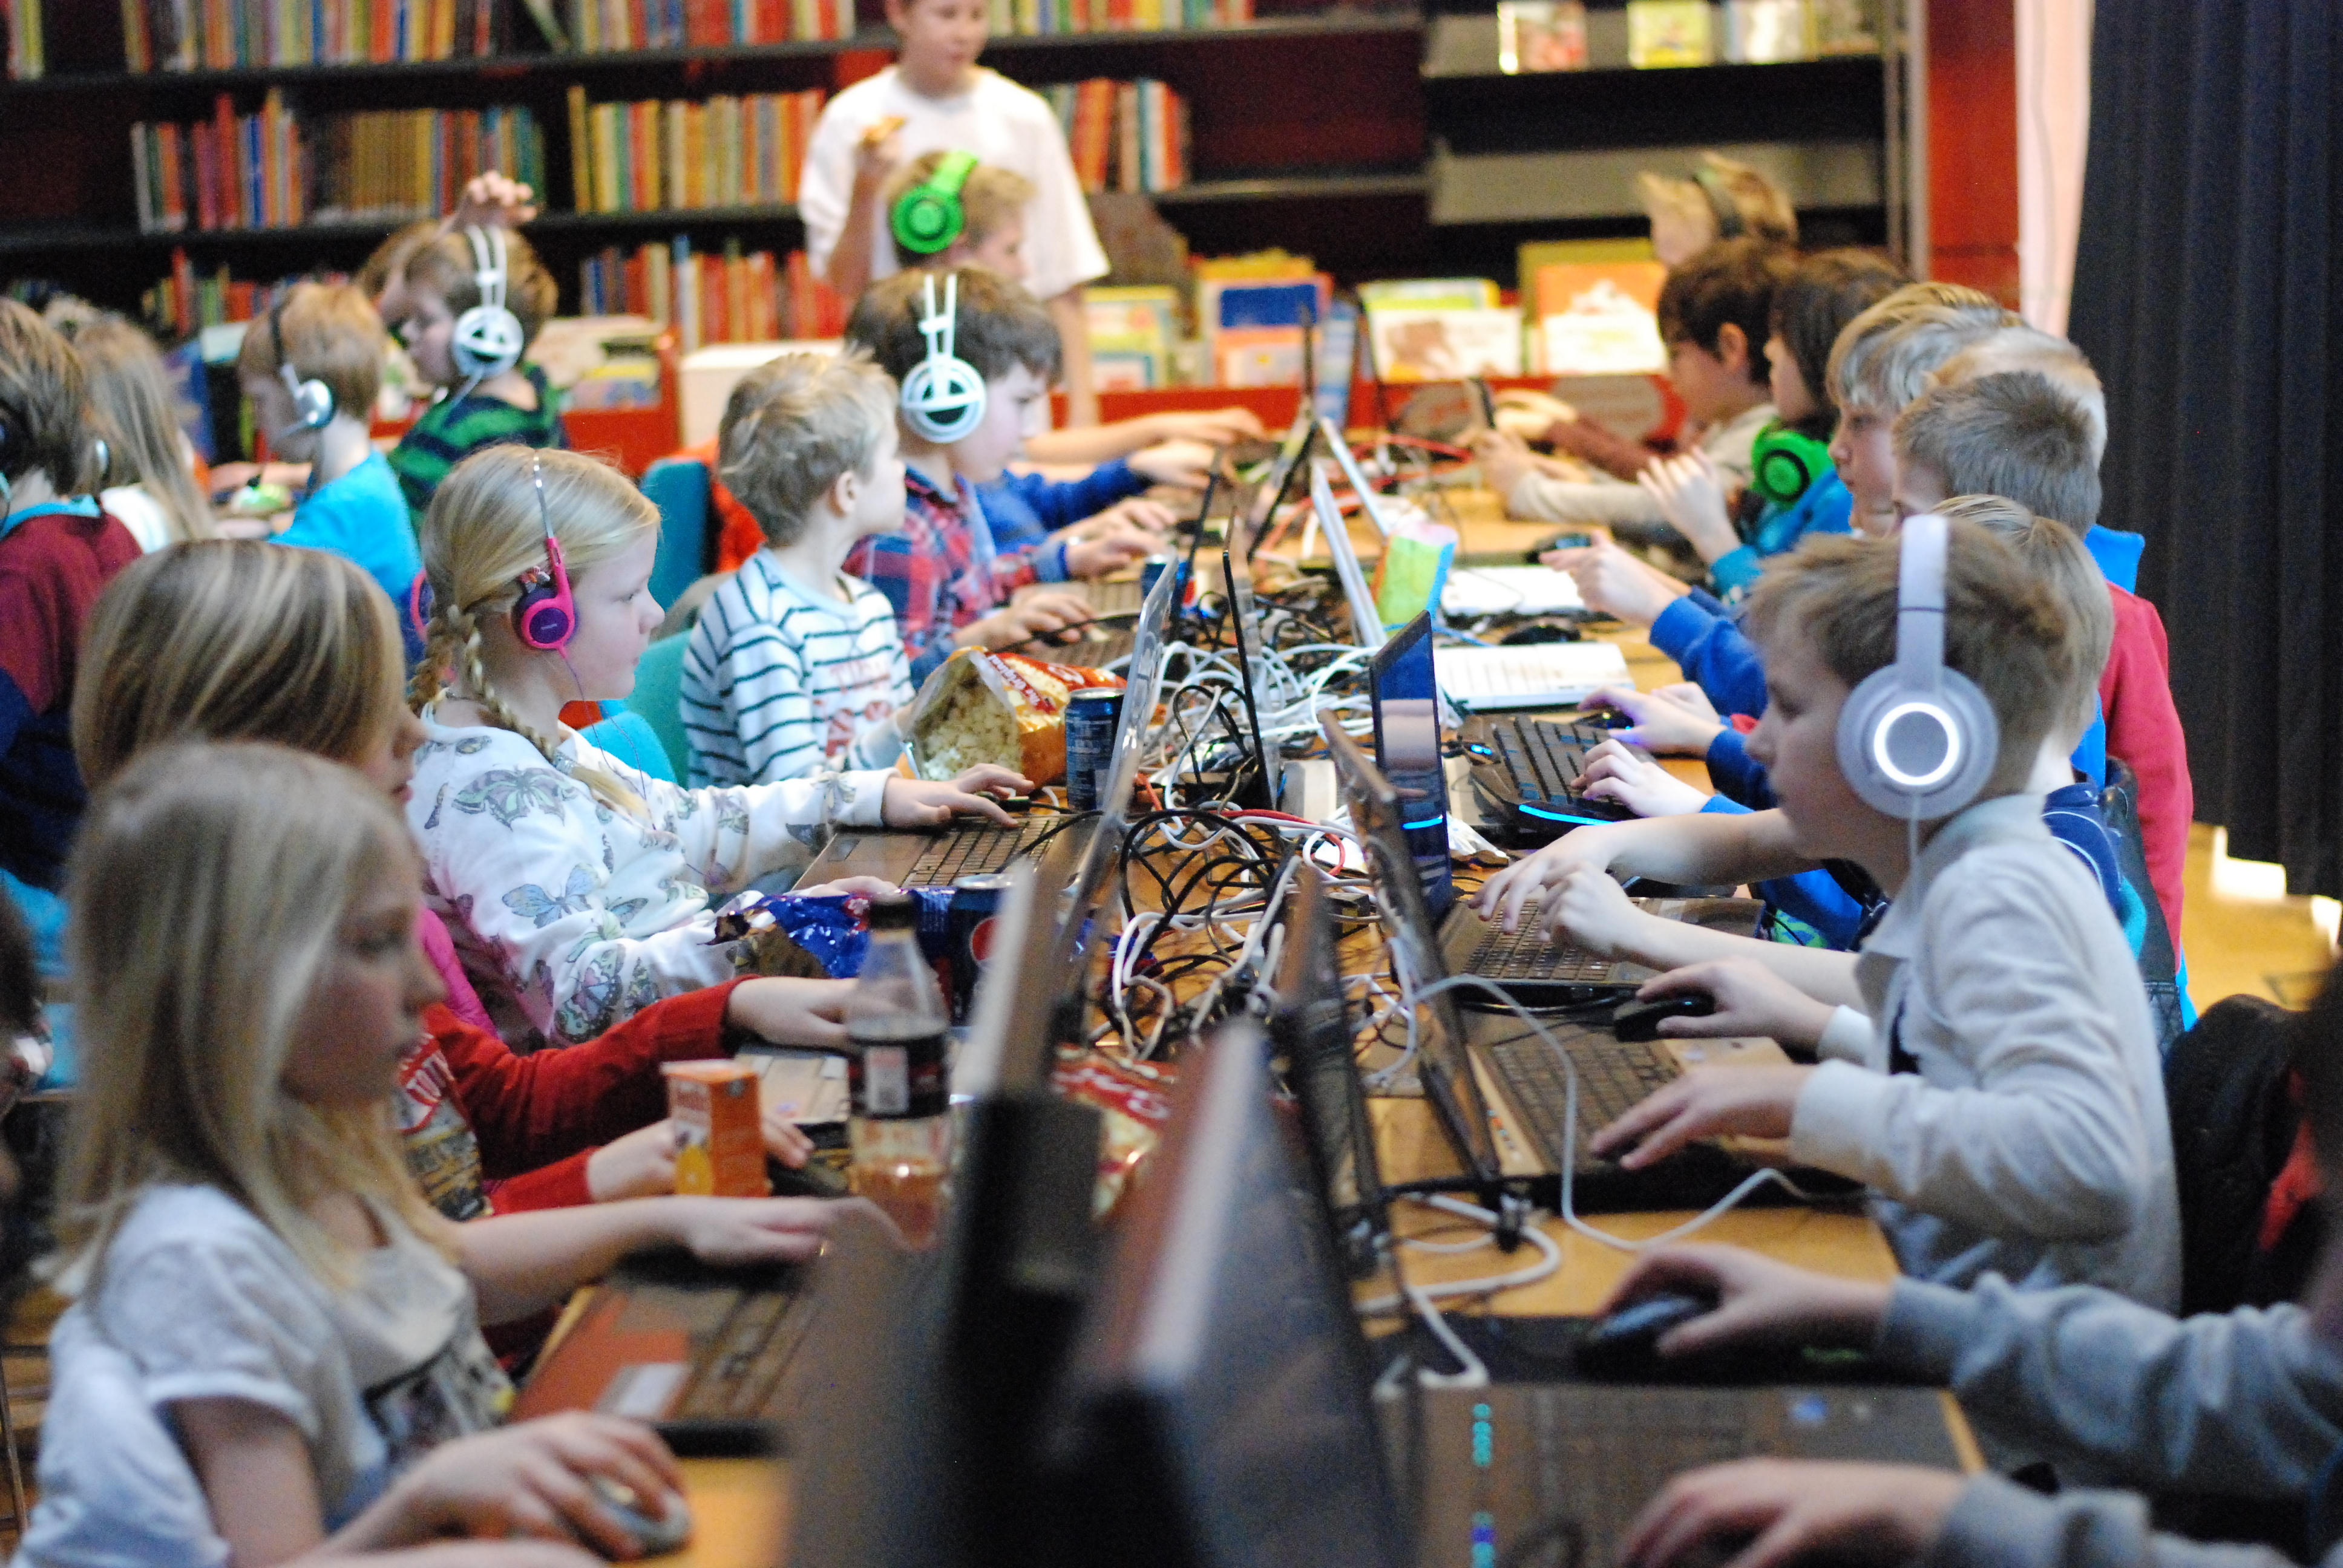
\includegraphics[height=1.2\paperheight]{Pictures/kids-programming}%
  };
  \end{tikzpicture}%
  \end{figure}%
  \end{frame}%


\begin{frame}[plain]
  \begin{figure}
  \centering
  \begin{tikzpicture}[overlay] 
  \node [] at (0.0mm,-5.0mm) {%
  \includegraphics[height=1.2\paperheight]{Pictures/titlepictureGroup}};
  \end{tikzpicture}%
  \end{figure}%
  \end{frame}%

\begin{Slide}{About our Scala students at Lund Univesity}
\begin{itemize}
\item Enrolled at the 5 year program in Computer Science \& Engineering (CSE) at LTH
\item Taking their first programming course 7.5 ECTS credits during their first semester
\item More than 80\% are 19--22 years old
\item Around 15\% are female     
\item 100\% are fluent in Swedish
\item Around 65\% have programmed before (C\#, Java, Python, Javascript, ...)
\item Very big span of pre-knowledge
\item Increasingly selective admission: 136 accepted out of 1337 applicants (2018)
\end{itemize}
\end{Slide}

\begin{Slide}{History of first languages at Lund University}
First languages for students of the Computer Science and Engineering (CSE) program:
\begin{table}
\begin{tabular}{c r | l l}
     & (Algol) & & (pre-history, starting with punch cards...) \\ & & \\
     & & 1982  & CSE program started at LTH\\ &  & \\
%\includegraphics[height=1.2em]{Pictures/pascal}  
&  { Pascal} & 1982--1989 & 8 years\\ &  & \\
%\includegraphics[height=1.2em]{Pictures/simula}  
&  { Simula} &  1990--1996 & 7 years \\
\includegraphics[height=2em]{Pictures/duke}    &  {\color{blue}\textbf{Java}} &  1997--2015 & 19 years \\
\includegraphics[height=2em]{Pictures/scala}   &  {\color{red}\textbf{Scala}} &  2016-- & \\
\end{tabular}
\end{table}

\end{Slide}

\begin{Slide}{The first year of the CSE program since 2016}
\begin{table}
\begin{tabular}{l| p{2.5cm} p{2.5cm} | p{2.5cm} p{2.5cm} }
  Semester & \multicolumn{2}{l}{Fall semester, 30hp } & \multicolumn{2}{|l}{Spring semester, 30hp} \\ \hline
  Period & 1 & 2 & 3 & 4 \\ 
  & \multicolumn{2}{c|}{\tikz{\node [draw, text width=5.22cm, align=center, fill=red!40] {\bf Programming 1 \newline (Scala) 7.5hp};}} 
  & \tikz{\node [draw, text width=2.5cm, align=center, fill=blue!30] {Progr. 2 (Java) 7.5hp };} 
  & \tikz{\node [draw, text width=2.5cm, align=center] {\small Discr. struct. (Closure) 5hp };} 
  \\
  & \tikz{\node [draw, text width=1.5cm, align=center, fill=green!20] {\small Computer intro. 3hp};} 
  & \tikz{\node [draw, text width=2.3cm, align=center] {\small Cognition 4.5hp};} 
  & \multicolumn{2}{c}{\tikz{\node [draw, text width=5.4cm, align=center] {\small Evaluation of software systems  (R) \newline 7hp};}} 
  \\
  & \multicolumn{2}{c|}{\tikz{\node [draw, text width=5.2cm, align=center] {\small Mathematics: \newline Calculus in one variable  \newline 15hp};}} 
  & \tikz{\node [draw, text width=2.5cm, align=center] {\small Physics: photonics 5hp};}
  & \tikz{\node [draw, text width=2.5cm, align=center] {\small Math: linear algebra 6hp};}
  \\
  
\end{tabular}
\end{table}  
{\small A study year is 60 ECTS higher education points (hp) = 40 weeks of full-time studies. }

\end{Slide}

\begin{Slide}{The Java first situation (2015)}
  I took over as course head of the first programming course in 2015 and ran it (almost) as usual with Java first, while in parallell heading the development of the Scala first course material as an open source community project with colleagues and senior students.

  \vspace{0.5em}%
  \begin{minipage}[t]{0.42\textwidth}
      \textbf{Good}:
      \begin{itemize}
        \item Course very popular
        \item Exam results very good:  
        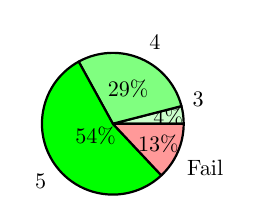
\begin{tikzpicture}[scale=0.3, every node/.style={scale=0.8}]
          \pie [color={green!20, green!50, green, red!40} ]  {4/3, 29/4, 54/5, 13/Fail}
          % inclding W {8/3, 28/4, 48/5, 16/Fail}
        \end{tikzpicture}
      
      \end{itemize}
    \end{minipage}%
    \begin{minipage}[t]{0.6\textwidth}
      \textbf{Bad}:
      \begin{itemize}
        %\item Some not so enthusiastic about Java         
        \item High-performing students not challenged
        \item Poor results in second course
      \end{itemize}   
    \end{minipage}
\end{Slide}

{
\begin{frame}[plain]
  \begin{tabular}{l | l | l | l | l }
   Grade &  Exam results &  &  & \\
   first & second course &  &  & \\
   course& 2015 {\color{blue}\textbf{Java}} first & 2016 {\color{red}\textbf{Scala}} first & 2017 {\color{red}\textbf{Scala}} first & 2018 {\color{red}\textbf{Scala}} first\\

   {\huge 3} & 
    \begin{minipage}{0.15\textwidth}%
      \centering%
      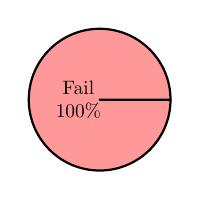
\begin{tikzpicture}[scale=0.3, every node/.style={scale=0.7}]
        \pie [color={green!40, red!40}, text=inside ] {0, 100/Fail}
      \end{tikzpicture}
    \end{minipage}%
     & 
     \begin{minipage}{0.15\textwidth}%
      \centering%
      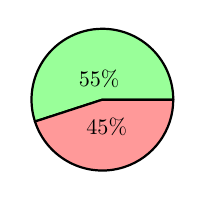
\begin{tikzpicture}[scale=0.3, every node/.style={scale=0.8}]
        \pie [color={green!40, red!40}, text= ] {55/Pass, 45/Fail}
      \end{tikzpicture}
    \end{minipage}%
    & 
    \begin{minipage}{0.15\textwidth}%
     \centering%
     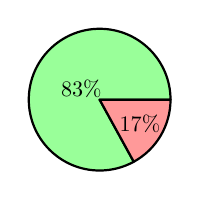
\begin{tikzpicture}[scale=0.3, every node/.style={scale=0.8}]
       \pie [color={green!40, red!40}, text= ] {83/Pass, 17/Fail}
     \end{tikzpicture}
   \end{minipage}%
   & 
   \begin{minipage}{0.15\textwidth}%
    \centering%
    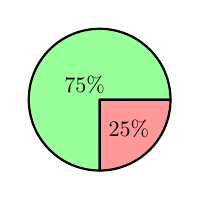
\begin{tikzpicture}[scale=0.3, every node/.style={scale=0.8}]
      \pie [color={green!40, red!40}, text= ] {75/Pass, 25/Fail}
    \end{tikzpicture}
  \end{minipage}%
  \\

     {\huge 4} & 
     \begin{minipage}{0.15\textwidth}%
       \centering%
       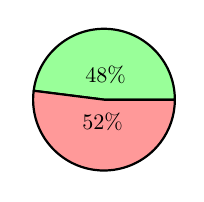
\begin{tikzpicture}[scale=0.3, every node/.style={scale=0.8}]
         \pie [color={green!40, red!40}, text= ] {48/Pass, 52/Fail}
       \end{tikzpicture}
     \end{minipage}%
      & 
      \begin{minipage}{0.15\textwidth}%
       \centering%
       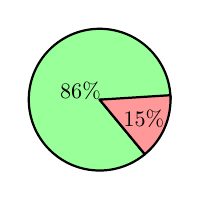
\begin{tikzpicture}[scale=0.3, every node/.style={scale=0.8}]
         \pie [color={green!40, red!40}, text= ] {86/Pass, 15/Fail}
       \end{tikzpicture}
     \end{minipage}%
     & 
     \begin{minipage}{0.15\textwidth}%
      \centering%
      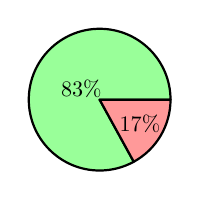
\begin{tikzpicture}[scale=0.3, every node/.style={scale=0.8}]
        \pie [color={green!40, red!40}, text= ] {83/Pass, 17/Fail}
      \end{tikzpicture}
    \end{minipage}%
    & 
    \begin{minipage}{0.15\textwidth}%
     \centering%
     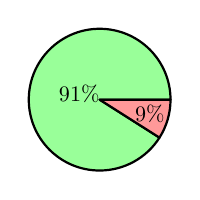
\begin{tikzpicture}[scale=0.3, every node/.style={scale=0.8}]
       \pie [color={green!40, red!40}, text= ] {91/Pass, 9/Fail}
     \end{tikzpicture}
   \end{minipage}%
     \\

      {\huge 5} & 
      \begin{minipage}{0.15\textwidth}%
        \centering%
        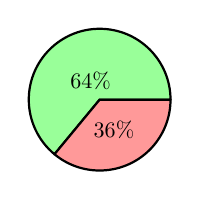
\begin{tikzpicture}[scale=0.3, every node/.style={scale=0.8}]
          \pie [color={green!40, red!40}, text= ] {64/Pass, 36/Fail}
        \end{tikzpicture}
      \end{minipage}%
       & 
       \begin{minipage}{0.15\textwidth}%
        \centering%
        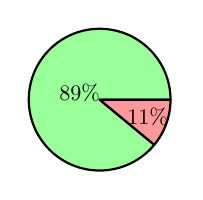
\begin{tikzpicture}[scale=0.3, every node/.style={scale=0.8}]
          \pie [color={green!40, red!40}, text= ] {89/Pass, 11/Fail}
        \end{tikzpicture}
      \end{minipage}%
      & 
      \begin{minipage}{0.15\textwidth}%
       \centering%
       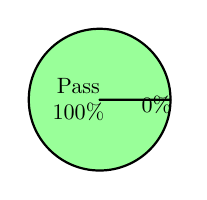
\begin{tikzpicture}[scale=0.3, every node/.style={scale=0.8}]
         \pie [color={green!40, red!40}, text=inside ] {100/Pass, 0/}
       \end{tikzpicture}
     \end{minipage}%
     & 
     \begin{minipage}{0.15\textwidth}%
      \centering%
      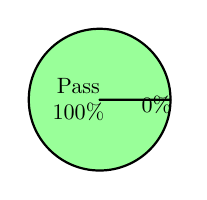
\begin{tikzpicture}[scale=0.3, every node/.style={scale=0.8}]
        \pie [color={green!40, red!40}, text=inside ] {100/Pass, 0/}
      \end{tikzpicture}
    \end{minipage}%
       \\

    \end{tabular}
\end{frame}
}

% \begin{Slide}{Our main goals of introducing Scala first}
%   \Large
%   \begin{enumerate}
%     \item Increase learning outcome for all students
%     \item Increase challenge level for high-performers 
%     %\item Increase collaborative learning
%   \end{enumerate}   
% \end{Slide}

\begin{Slide}{Scala first -- a big success! \texttt{~:)}}
\begin{itemize}
  \item Exam results in second course much better: increased learning outcome
  \item Course evaluations are still very positive: increased student engagement
  \item All students are challenged, independent of pre-knowledge
  \item Students find Scala interesting and novel
  \item Exam results: \\\vspace{0.5em} 
  \begin{tabular}{l l l}
  2016 & 2017 & 2018 \\
  \begin{minipage}{0.27\textwidth}%
    \centering%
    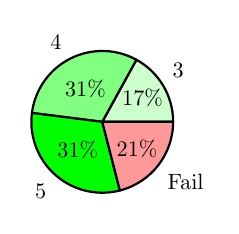
\begin{tikzpicture}[scale=0.3, every node/.style={scale=0.8}]
      \pie [color={green!20, green!50, green, red!40} ]  {17/3, 31/4, 31/5, 21/Fail}
    \end{tikzpicture}
\end{minipage}%
  & 
  \begin{minipage}{0.27\textwidth}%
   \centering%
   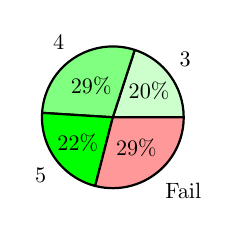
\begin{tikzpicture}[scale=0.3, every node/.style={scale=0.8}]
    \pie [color={green!20, green!50, green, red!40} ]  {20/3, 29/4, 22/5, 29/Fail}
  \end{tikzpicture}
\end{minipage}%
 & 
 \begin{minipage}{0.27\textwidth}%
  \centering%
  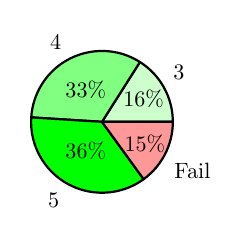
\begin{tikzpicture}[scale=0.3, every node/.style={scale=0.8}]
    \pie [color={green!20, green!50, green, red!40} ]  {16/3, 33/4, 36/5, 15/Fail}
  \end{tikzpicture}
\end{minipage}%
   \\

  \end{tabular}
\end{itemize}

\end{Slide}



\Section{How did we implement Scala first?}

\begin{Slide}{Pedadogical ideas behind course design}

  \begin{minipage}{0.22\textwidth}
    \includegraphics[height=0.52\textheight]{Pictures/marton}\\
    {\small Marton \& Tsui (2004)}
  \end{minipage}%
  \begin{minipage}{0.3\textwidth}
      Patterns of variation:
      \begin{itemize}
        \item contrast
        \item generalize
        \item separate
        \item fuse
      \end{itemize}
  \end{minipage}%
  \begin{minipage}{0.22\textwidth}
      \includegraphics[height=0.52\textheight]{Pictures/brown}\\
      {\small Brown et al. (2014)}
    \end{minipage}%
    \begin{minipage}{0.25\textwidth}
        Easier isn't better: \\        
        embrace desirable\\difficulties!
    \end{minipage}
\end{Slide}



\begin{Slide}{A typical study week}
 % Resources for 135 students: 1 lecturer (me), 14 teaching assistants (older students). 
\begin{table}\centering
  \begin{tabular}{l | l |l l | l}
  Mon & Tue & Wed & Thu & Fri \\ \hline
  Lecture (2h) & Lecture (2h) & \multicolumn{2}{c|}{Workshop (2h)} & Lab session (2h) \\ \hline
  \end{tabular}
\end{table}
  \begin{itemize}
    \item Workshops and labs in computer rooms with Ubuntu \& pre-installed Scala tools 
    \item Workshops focus on work with \textbf{exercises} on concepts related to weekly \textbf{theme}. 
    \item 7 workshop time slots (2h) per week in 2 computer rooms in parallell. 
    %\item If there is space left in room you can attend several workshops.
    \item 2 \textbf{lab} time slots (2h) per week in 6 rooms in parallell. Labs are assessed pass/fail.
    %\item Computer rooms are available to students 24/7 when no teaching is scheduled.
    %\item Link to full schedule: \url{http://cs.lth.se/pgk/schema/}
  \end{itemize}
\end{Slide}  

\begin{Slide}{How did we design contents \& progression?}
  \begin{minipage}{0.55\textwidth}
    \fontsize{8.7}{10}\selectfont
    % \begin{tabular}{|l|l|l|}
    %   \textit{Week} & \textit{Main Theme} & \textit{Lab} \\ \hline \hline
    %   W01 & Introduction    & kojo \\
    %   W02 & Programs        & -- \\
    %   W03 & Functions       & irritext \\
    %   W04 & Objects         & blockmole \\
    %   W05 & Classes         & blockbattle \\
    %   W06 & Sequences       & shuffle \\
    %   W07 & Sets, Maps      & words \\ \hline 
    %       & Diagnostic test & -- \\ \hline
    %   W08 & Matrices        & life \\
    %   W09 & Inheritance     & snake \\
    %   W10 & Patterns        & tabular \\
    %   W11 & Scala \& Java   & javatext \\
    %   W12 & Sorting         & -- \\
    %   W13 & Projekt         & Projekt \\
    %   W14 & Exam prep.      & \\ \hline
    %       & Written exam    &  \\ 
    %   \end{tabular}  
    \begin{tabular}{|l|l|l|l|} 
      \textit{Week} & \textit{Main Theme} & \textit{Lab} & \textit{Tools}\\ \hline \hline
      W01 & Expressions     & kojo        & Kojo, REPL\\
      W02 & Programs        & --          & vscode, scalac\\
      W03 & Functions       & irritext    & sbt\\
      W04 & Objects         & blockmole   & introprog-scalalib\\
      W05 & Classes         & --          & \\
      W06 & Patterns        & blockbattle & \\
      W07 & Sequences       &  shuffle    & \\ \hline 
      \multicolumn{2}{r}{\textit{Exam period:}} & \multicolumn{2}{l}{\textit{Diagnostic test}} \\ \hline
      W08 & Matrices        & life        & IDE: IntelliJ (opt.)\\
      W09 & Sets, Maps      & words       & \\
      W10 & Inheritance     & snake       & \\
      W11 & Scala \& Java   & javatext    & \\
      W12 & Search \& Sort  & --          & \\
      W13 & Projekt         & Projekt     & \\
      W14 & Exam prep.      &             & \\ \hline
      \multicolumn{2}{r}{\textit{Exam period:}} & \multicolumn{2}{l}{\textit{Final exam}} \\ \hline
      \end{tabular}  

  \end{minipage}%
    \begin{minipage}{0.31\textwidth}
      {\hspace{0.5em} Teaching material:}
      \begin{itemize}
        %\item Progression is based on experiences 2016-2018 
        \item Lecture slides and \textbf{compendium} with weekly assignments %(exercises \& labs)
        %\\ https://github.com/lunduniversity/introprog
        \item Simple Scala lib with pixel window, io etc.: {github.com/lunduniversity/\\\textbf{introprog-scalalib}}
        \item All material is open source {\footnotesize CC-BY-SA} developed  together with senior students
      \end{itemize}
    \end{minipage}%
    \tikz[overlay]{\node [text width=2.1cm, align=left] at (1,1.65) {\includegraphics[width=1.0\textwidth]{Pictures/compendium}};} 
  \end{Slide}

\begin{Slide}{How did we deal with a very broad spectrum of pre-knowledge?}
  The challenge level in assignements are variable: 
  \begin{itemize}
    \item All exercises have three parts 
    \begin{itemize}
      \item Foundation task: exercise the concepts of this week 
      \item Extra tasks: variations, if you need more training
      \item Advanced tasks: go deeper and beyond
    \end{itemize}
    \item All labs have two parts:   
    \begin{itemize}
      \item Mandatory task: makes your program work 
      \item Elective tasks: add interesting features to your program 
    \end{itemize}  
  \end{itemize}
\end{Slide}

\begin{Slide}{The first three weeks are playful}
  
  \begin{itemize}
    \item Computing course in parallel: intro to Linux terminal on school computers (Ubuntu)
    \item Student's traditional freshman games and festivities in parallell
    \item []
    \item \textbf{Week 1}: Intro to basics using expressions in REPL and turtle graphics in Kojo; \textbf{S}equencing, \textbf{A}lternative, \textbf{R}epetition, \textbf{A}bstraction (SARA)%: \url{http://www.kogics.net/kojo-download}: \\ Working with expressions in REPL and control flow principles (SARA) in Kojo: 
    \begin{minipage}{0.3\textwidth}
      
    \end{minipage} 
 
    \item \textbf{Week 2}: Small readln println programs using editor (VS Code + Metals).\\ Compile in terminal with \code|scalac|, run with \code|scala|
      
    \item \textbf{Week 3}: Create a \textit{lagom} irritating terminal text game at your challenge level, focus on readability of your code.\\ 
      
      Compile \& run with \code|sbt ~run| , you should divide your code into several functions.   
  \end{itemize}
\footnotesize{https://en.wikipedia.org/wiki/\textbf{Lagom} \\ Swedish for ''\textbf{just right}'', carries the connotation of appropriateness, although not necessarily perfection}
\end{Slide}  


\begin{Slide}{A first understanding of basic concepts (SARA)}
\begin{minipage}{0.6\textwidth}
\includegraphics[width=0.9\textwidth]{Pictures/kojo-en}  
\end{minipage}%
\begin{minipage}{0.4\textwidth}
 \includegraphics[width=0.15\textwidth]{Pictures/square}%
 \includegraphics[width=0.25\textwidth]{Pictures/square-column}%
 \includegraphics[width=0.5\textwidth]{Pictures/square-grid}  \\
 \vfill{http://www.kogics.net/kojo}
\end{minipage}%
\end{Slide}  
  


\begin{Slide}{Continuous assessment: Lab sessions}
  \begin{tabular}{c c c c}
    W04: \textbf{blockmole} & W06: \textbf{blockbattle} & W08: \textbf{life} & W10: \textbf{snake} \\
  \includegraphics[width=0.2\textwidth]{Pictures/blockmole} &
  \includegraphics[width=0.15\textwidth]{Pictures/blockbattle} &
  \includegraphics[width=0.27\textwidth]{Pictures/life} &
  \includegraphics[width=0.25\textwidth]{Pictures/snake} 
  \\
  \small val, var, function, & \small class, case class & \small nested structures, & \small inheritance, \\
  \small object, name space, & \small match, pattern, & \small higher order fun, & \small interface, override, \\
  \small import, if else if else & \small a larger program & \small generic case class & \small team work\\
\end{tabular}%
\end{Slide}  

% \begin{Slide}{Mid term diagnostic test: progress check}
%   \begin{itemize}
%     \item same format as final exam, but half as big, 2.5 h
%     \item peer marking
%     \item confirm that you are on track
%     \item early warning for some
%   \end{itemize}
% \end{Slide}  


% \begin{Slide}{Final exam: securing the learning outcome}
%   5h written hall exam using pen and paper and Scala quick ref only
% \end{Slide}  


\Section{What did we learn?}


\begin{Slide}{Experiences with Scala first -- Benefits}
  My hypotheses supported by my experience since 2011 (but no systematic empiricism):
  \begin{enumerate}
  \item Scala can be simple enough for beginners \textit{and} interesting for non-beginners %(depending how you teach...)
  \item Scala is exciting to both students \& teachers: a modern language -- you can grow 
  \item Regular semantics is easier for beginners; e.g. value types are real objects
  \item Ability to do interesting things with small programs is important for beginners
  \begin{itemize}
    \item Scala is expressive and concise (but not too concise) 
    \item Scala has a simple-to-learn, powerful, regular, simple-to-use standard library
  \end{itemize}
  \item Static typing better for beginner debuggers: the Scala compiler is your friend  
  \item Beginners understand concepts step by step: iterative learning in the Scala REPL  
  %\item Rich semantics: can demonstrate many computer science concepts

  %\item Free, open source language and tools: no vendor lock-in (cf. .net, Swift)
  \item Multi-paradigm: allows for contrasting important ideas; contrasting helps learning
  \item Ability to do things in several ways help deeper conceptual knowledge building
  \end{enumerate}  
\end{Slide}


\begin{Slide}{Experiences with Scala first -- Challenges}
  Things we have struggled with in a trial \& error fashion:
  \begin{enumerate}
  \item Developing \textbf{teaching material} for Scala from scratch that \textbf{fit our context} \\ {\footnotesize Our CSE students seem less enthusiastic about learning from text books...}
  
  \item Selecting a \textbf{lagom subset} of Scala 
  \begin{itemize}
    \item pitfalls: including to many concepts; in-coherent progression 
    \item examples of what we excluded: \\creating type classes, recursive data types, recursive algorithms 
   \end{itemize}  
  \item Designing an \textbf{effective progression} with step-wise iteration of concepts combined
  %\item Complete beginners stumble on getting tooling to work on their own machines
  \item Helping beginners to overcome \textbf{tool barriers} (editor, compiler, build tool, IDE)
  \end{enumerate}  
\end{Slide}


\begin{Slide}{Key ingredients in our progression for Scala first}
 \begin{enumerate}
 \item  Introduce concepts iteratively: first separated, then combined,  use variation patterns  
 \item Initial playful assignments to illustrate programming (e.g. using turtle graphics)
 \item Start with expressions and simple functions in REPL, then small but complete imperative programs compiled in terminal: manifest mental model of execution
  \item Objects are introduced as modules to create name space
  \item Classes are introduced to enable multiple instances
  \item Case classes introduced together with general classes: \\
   contrast immutable and mutable state; use patterns to deconstruct data
  \item Inheritance introduced iteratively, start with simple sum type (base trait + case object)
  \item Progression of collections: sequences (Vector, Array), nested sequences, Set, Map 
  \item Power of higher-order functions experienced through the collection library
\end{enumerate}
\end{Slide}  


\begin{Slide}{How did we mix OO and FP in our teaching?}
  Scala's OO+FP mix enables learning by concept awareness and patterns of variation:
  \begin{enumerate}
    \item Awareness of types of values, expressions, parameters, return types
    \item Contrast mutable state (class with var) -- immutable data (case class)
    \item Contrast inheritance for modelling -- inheritance for reuse
    \item Contrast side-effecting functions -- referentially transparent functions
    \item Contrast inheritance -- composition -- state-less modules of functions
  \end{enumerate}
\end{Slide}  


\Section{The road ahead}

\begin{Slide}{The future of Scala at Lund University}
\begin{itemize}
  \item CSE students strongly support Scala first; course evaluations are excellent
  \item There is a great interest among CSE students to continue with Scala in later courses; this depends on if more cs teachers want to learn and try out Scala 
  \item Hopefully more IT programs that currently have Java first are attracted to the new pedagogical concept of the CSE course
  \item On-going debate of pros and cons of Scala first versus Python first for non-IT programs, e.g. chemistry, physics, civil engineering etc.
\end{itemize}  
\vfill \url{https://www.signifytechnology.com/blog/2018/06/supporting-scala-adoption-in-colleges-by-mark-lewis}
\end{Slide}

\begin{Slide}{Scala: A better deal for beginner programmers?}
  \begin{itemize}
    \item Scala 3 for beginners: opportunity to show-case idioms for \textit{the \textbf{simple} parts}
    %\item Spreading the news of Scala turning main-stream 
    \item Join forces for high-quality open source \textbf{beginner teaching material}
    \item A beginner-friendly library for \textbf{analyzing data} in .csv (as easy as MatLab, numPy, R)
    \item Improve official \textbf{scripting} model (cf. ammonite: scripts calling scripts, ivy import)
    \item Better \textbf{tooling UX} for beginners: 
    \begin{itemize}
      \item Better \textit{desktop} coding experience for \textbf{university} students: one single-click install of signed snap \& .msi \& .dmg  complete Scala bundle (REPL in terminal, vs code, intellij scala bundle) available in desktop official app stores for linux, windows and mac
      \item Better \textit{browser} coding experience for \textbf{primary school} students: single click browser client js app with compiler running under Scala.js compiling to local store not needing network connection after download available as signed app in app stores for ChromeOS, IOS, Android
    \end{itemize}
  \end{itemize}

\end{Slide}

%%%%%%%%%%%%%%%%%%%%%%%%%%%%%%%%%%%%%%%%%%%%%%%%%%%%%%%%%%%%%

\begin{frame}[plain]
  \begin{figure}
  \centering
  \begin{tikzpicture}[overlay] 
  \node [] at (0.0mm,-15.0mm) {%
    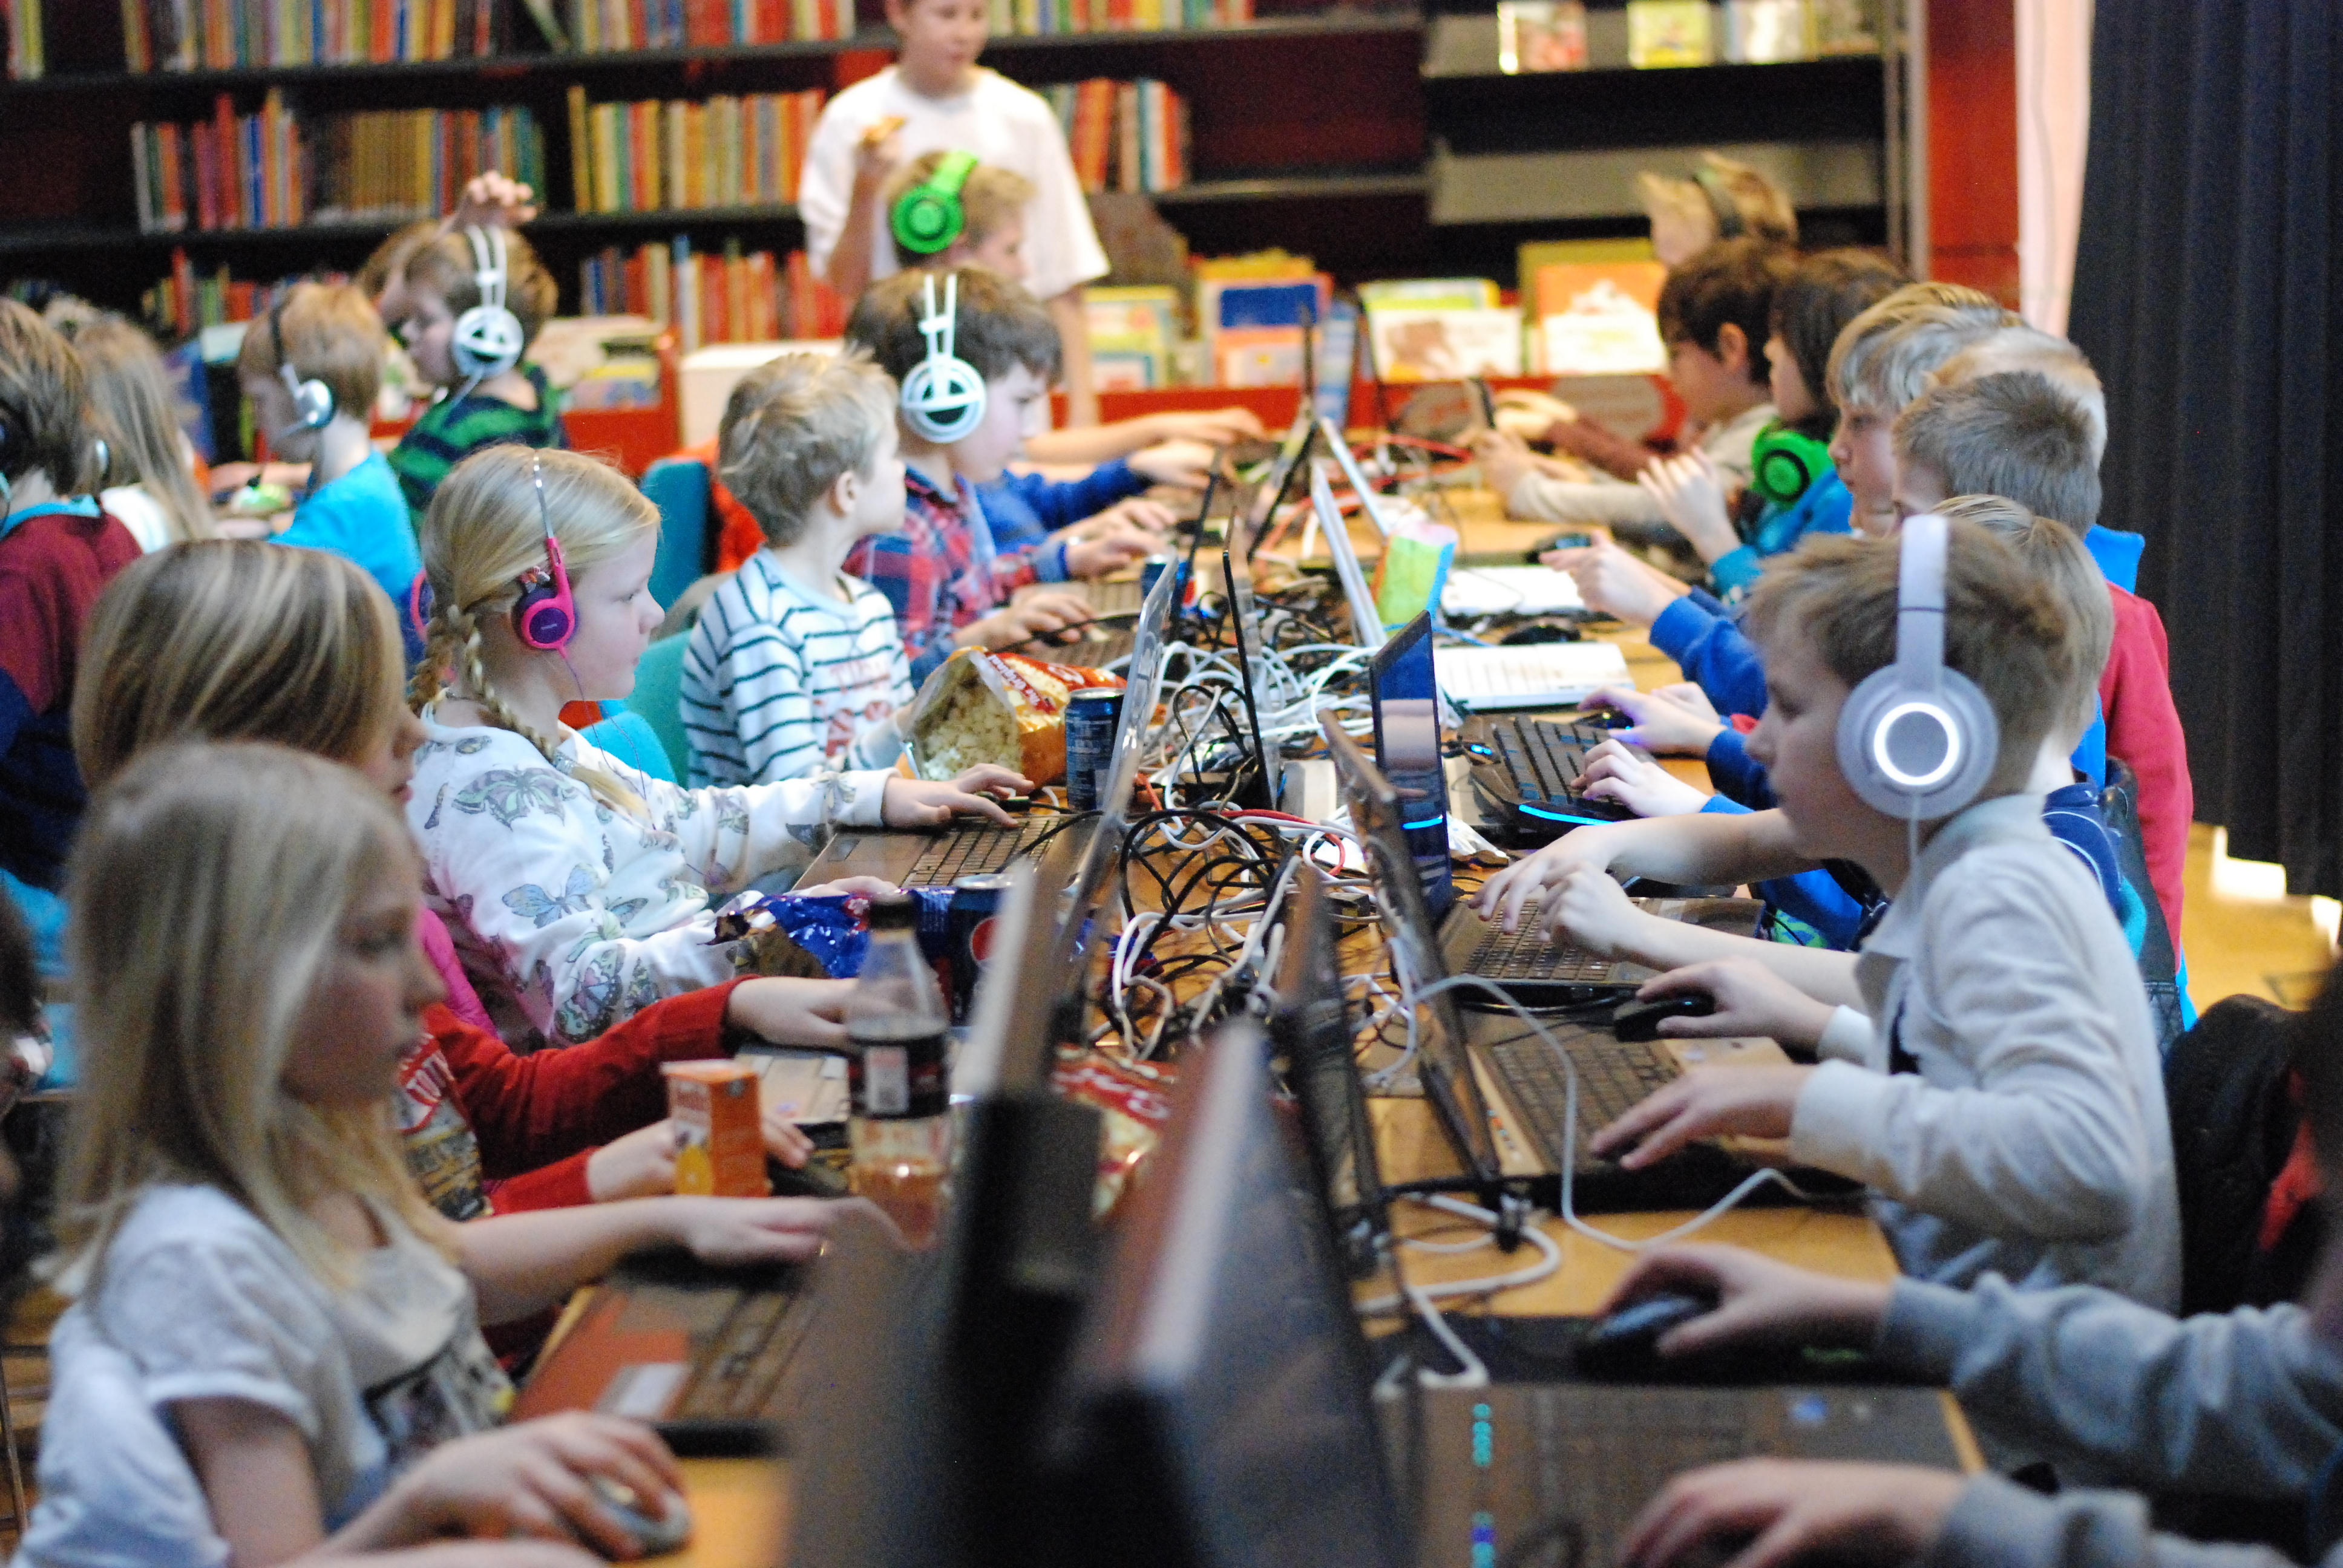
\includegraphics[height=1.2\paperheight]{Pictures/kids-programming.JPG}%
  };
  \end{tikzpicture}%
  \end{figure}%
  % \tikz[overlay]{
  %   \node [] at (0.5\paperwidth,0.0cm) {\includegraphics[height=5cm]{Pictures/scala}};
  % }

  \tikz[overlay]{
    \node [] at (0.45\paperwidth,-3.5cm) {\color{white!40}{\fontsize{16}{16}\selectfont\bf Next Gen Devs}};
  }

\end{frame}%


\EndSlide

%Slides that didn't make due to time limit

\begin{Slide}{Why not Python first?}
  My hypotheses based on some experience (but no systematic empiricism):
\begin{itemize}
  \item Dynamic typing means less help in finding bugs
  \item No ''typing dialog'' with a compiler means less conceptual learning
  \item Non-explicit types in function defs is less efficient when learning abstract thinking
  \item Indentation syntax with silent begin-end makes nested blocks obscure to beginners
  \item No explicit variable declaration can lead to very hard bugs also for non-beginners 
  \item Refactoring is more risky, hence discouraging -> bad for stepwise problem solving
  \item Not excellent at object orientation
  \item Not excellent at functional programming
\end{itemize}  
\end{Slide}


\begin{Slide}{Teaching benefits of a multi-paradigm language}
  \begin{minipage}{0.2\textwidth}
    \includegraphics[height=0.52\textheight]{Pictures/marton}\\
    {\small Marton \& Tsui \newline (2004)}
  \end{minipage}%
  \begin{minipage}{0.85\textwidth}
    \begin{itemize}
      \item Learning is the process of being capable of \textit{doing} something
      \item Learners construct a language by discerning parts and wholes % that are experienced in context   
      \item Patterns of variation:
      \begin{itemize}
        \item \textbf{Contrast}: to experience something, you need to experience something else to compare with    
        \item \textbf{Generalisation}: to understand a concept you need to be able to abstract from irrelevant features    
        \item \textbf{Separation}: to experience a certain aspect of something, you need to vary that aspect while other aspects remain fixed    
        \item \textbf{Fusion}: to be capable of doing something advanced you need to experience several critical aspects at the same time    
      \end{itemize}
    \end{itemize}
  \end{minipage}
  
  \vspace{1em} Scala enables contrasting, generalisation, separation and fusion across paradigms.
  
  \end{Slide}
  
  \begin{Slide}{Pedagogical ideas behind course design}
    \begin{minipage}{0.3\textwidth}
      \includegraphics[height=0.6\textheight]{Pictures/brown}\\
      Brown et al. (2014)
    \end{minipage}%
    \begin{minipage}{0.7\textwidth}
      A great summary of research on effective learning strategies:
      \begin{itemize}
        \item How learning occurs: encoding, consolidation, retrieval
        \item Low-stake self testing to retrieve what you learned and identify missing pieces
        \item Deliberate practice: spaced out \& interleaved
        \item Use reflection \& elaboration as you retrieve
        \item Easier isn't better: embrace desirable difficulties
        \item How effort helps: reconsolidation, creating mental models, broaden mastery, foster conceptual learning, improve versatility, prime your mind for learning 
        \item Dismissed myths: errorless learning, learning styles
      \end{itemize}
    \end{minipage}
    \end{Slide}
  
\EndSlide


\end{document}